\chapter{On the Resurrection of Jesus}\label{ch:resurrection}
%!TEX root = main.tex

\section{Is the resurrection 97\% likely?}

Richard Swinburne has written\cite{swinburne2004existence,swinburne2003resurrection} that a thorough probabilistic approach leads one to the conclusion that the resurrection is at least 97\% likely.  His argument is summarized here.  He defines a number of propositions.

\bi
\i $t$: theism is true - there is a God (of the traditional kind)
\i $k$: background knowledge of natural theology
\i $P(t|k)$: probability there is a God (of the traditional kind) given the background knowledge of natural theology.  He suggests (from Chapter 1) a ``modest'' value of
\[
P(t|k) = 1/2
\]
\i $c$: the claim God became incarnate at some time
\i $P(c|t,k)$: probability that ``God became incarnate at some time'' given that ``there is a God (of the traditional kind)'' and ``the background knowledge of natural theology''  Again, from (Chapter 2) he suggests a ``modest'' value of
\[
P(c|t,k) = 1/2\]
\i $P(c|k)$: probability that ``some God became incarnate at some time'' given ``the background knowledge of natural theology''.  Mathematically it is related to the other terms as
\[
P(c|k)= P(c|t,k) \times P(t|k) = 1/2\times 1/2 = 1/4
\]
\i $e$: historical evidence, broken up into
    \bi
    \i $e_{1}$: evidence of the life of Jesus (Part II)
    \i $e_{2}$: evidence of the detailed history of the Resurrection (Part III)
    \i $e_{3}$: evidence that Jesus satisfies the requirements for divine incarnation more than other prophets (Chapter 3)
    \ei
\i $f$: claims that the evidence of the strength given by $e$ (also broken up into $f_{1}$, $f_{2}$, and $f_{3}$
\i $P(c|f,k)$: the probability of the incarnate God, given the evidence.  This is the term that Swinburne is ultimately interested in.  His final result is
\[
P(c|f,k) = \frac{100}{103} = 0.97
\]
We'll see how he gets there as we continue.
\i $P(f|c,k)$: the probability that, if God became incarnate, we would have the evidence we have.  Swinburne suggests the ``fairly low'' number of $P(f|c,k) = 1/10$
\ei
Now all we need do is apply the rules of probability from these estimates, and we obtain Swinburnes answer of 97\% probability that God became incarnate in Jesus given the evidence,
\beqn
P(c|f,k) &=& \frac{P(f|c,k) P(c|k)}{P(f|k)}\\
P(c|f,k) &=& \frac{P(f|c,k) P(c|k)}{P(f|c,k) P(c|k) + P(f|\sim(c,k)) P(\sim c|k)}\\
&=& \frac{\frac{1}{10}\times \frac{1}{4}}{\frac{1}{40} + \left(\frac{3}{4}\times\frac{1}{1000}\right)} \\
&=& 0.97
\eeqn

In his book on the existence of God, Swinburne provides a series of pieces of evidence, denoted $e_{n}$, where $P(e_{n}|h,k)>P(e_{n}|k)$ or the evidence is more likely with theism than in just the background.  He does, however, state that added assumptions to $h$ must be added to account for some pieces of evidence of evil that are less likely under, what he calls, ``bare theism''.  

\pquote{The fact that the [evidence of] evil required additional hypotheses to be added to the hypothesis of theism to save it from disconfirmation meant that the evil
lowered the probability of theism as such (bare theism) from its probability on the evidence taken into account previously. The fact of divine hiddenness did not, how- ever, count against the existence of God.}

Swinburne's calculation follows Bayes' rule

\beqn
P(h|e,k) &=& \frac{P(e|h,k)P(h|k)}{P(e|h,k)P(h|k)+P(e|\sim h,k)P(\sim h|k)}
\eeqn

\pquote{Let us turn now to $h_{2}$. This is the hypothesis that there is no god or gods, but an initial or everlasting physical state of the universe, different from the present state but such as to bring about the present state. But there is no particular reason why an unextended physical point or any of the other possible starting points of the universe, or an everlasting extended universe, should as such have the power and liability to bring about all the features that I have described.}

\bi
\i e1 be ?there is a physical universe?.
\i second argument, from e2 (which will be the conformity of the universe to temporal order) i.e. subject to temporal order
\i e3, etc.. consciousness, morality
\ei

No physical model here, just words.

\pquote{Now I suggest that a universe without connections between uni- versals would be simpler than one with connections; and one with simpler patterns of connection would be simpler than one with such complicated patterns of connection that rational beings would not be able to infer the future behaviour of objects by means of the simplest extrapolation from their past behaviour. Among theories of the universe as a whole (which will thus have equal scope), simplicity is the sole indicator of intrinsic probability. It then follows that, if we give it the weight that I have urged that we should (so that a very simple theory is more probable than a disjunction of many more complex theories), it would be very probable that there would be no connections between universals at all?that the universe would be chaotic....Either way, it is going to be improbable that in a Godless universe there will be simple connections between universals, and so simple laws of nature. }

\pquote{The arguments of the previous pages have sought to show just this; and indeed that the probability of order of the right kind is very much greater if there is a God, and so that the existence of such order adds greatly to the probability that there is a God.}


\pquote{If only a very narrow range of laws and initial conditions allow such evolution, then we may say that the universe is ?fine-tuned? for this evolution.}

\pquote{There remains, however, a consensus among physicists that the values of the constants in the laws of standard theory (as opposed to the variables of initial conditions) must lie within very narrow ranges if life is to evolve anywhere in the universe?ranges that include the actual values of the constants and probably a few other small ranges in which the values of several of the constants are different from their actual ones. }

\pquote{But the considerable a priori weight of simplicity suggests that in a Godless universe it is a priori improbable that any one universe will be tuned so as to yield human bodies. With $e$ as the existence of human bodies, $h$ as theism, and $k$ as the evidence of a universe conforming to natural laws, $P(e|\sim h,k)$ is very low.}

\pquote{The laws of Relativity Theory and Quantum Theory, integrated perhaps into a ?Grand Unified Theory? or ?Theory of Everything? by which everything physical might be explained (fully or partially, even if not complete- ly), give not the slightest reason to suppose that some brain state would cause a green sensation or a sensed smell of coffee.}

\pquote{If, when I tried to move my foot, my hand moved instead, predators would soon overtake me. But this correct explanation of why (given that intentions cause brain events) the brain is connected by nerves to the rest of the body in the way it is does not explain why we have intentions to move our bodies at all and why they cause brain events, which is a quite different problem. I conclude that the existence of the most novel and striking features of animals and above all of humans (their conscious life of feeling, choice, and reason, causing connected to their bodies) seems to lie utterly beyond the range of successful scientific explanation.}

How is this possible?  

\pquote{I argued in Chapter 6 that there was a significant probability to which I gave the somewhat artificial value of 1/2 that a God would create humanly free agents?that is, beings who could choose how to make important differences to themselves, each other, and the world.}


\pquote{I have been arguing that, by permitting moral evil and bringing about natural evil, God gives us (and animals) a good that he could not give us in any other morally permissible way.}

\pquote{Hence evil provides a good C-inductive argument against the existence of God. But it does not provide a very strong one, for the reason that providing life after death for many humans (not merely those who need compensation) and becoming incarnate to share their suffering are the kinds of act that a good God might well do anyway?for they are good acts (and perhaps good acts of different kinds from the other acts of God that we have been discussing, and maybe even acts of best kinds), whether or not required in order for God justifiably to allow the amount of evil that occurs. (See p. 231 for the goodness of an act of the former kind, and pp. 288?90 for additional reasons that God might have for becoming incarnate.) So, with e as the occurrence of the moral and natural evils known to us, h as the hypothesis of theism, and k as the evidence considered in previous chapters, $P(h|e , k) < P(h|k)$, but the former is not less than the latter by very much.}

Argument from divine hiddenness

\pquote{But, if the good desire is stronger than the bad one and I have a deep awareness of the presence of God (that is, such that God?s existence is not open to question), then the balance of inclination will be to the good and there will be no free choice between good and bad. We will be in the situation of the child in the nursery who knows that mother is looking in at the door, and for whom, in view of the child?s desire for mother?s approval, the temptation to wrongdoing is simply overborne. We need ?epistemic distance? from God in order to have a free choice between good and evil.}

Miracles

\pquote{But although God has reason for bringing these things about, he also has reason for not bringing them about or not bringing them about too automatically in response to human needs....The major such reason is that it is good that humans should decide for themselves whether to warn or convert others, that humans should have some responsibility for the (immediate or long-term) spiritual destiny of their fellows. }

\pquote{My conclusion to this section is that, in so far as we have historical evidence (normally in the form of testimony) to the occurrence of an event E that is such that, if it occurred, it would probably be a violation of natural laws and that is of a kind that there is some probability that a God would have reason to bring about, that makes it more probable than it would otherwise be that there is a God. For a God would be expected occasionally to bring about such events. Yet, if there is no God, there is no significant probability that such events will occur. Evidence that an event is of this kind is evidence that it is an event ?too odd? for science to explain. Hence, with k as the evidence discussed in previous chapters, and e as evidence of testi- mony of the above kind, and h the hypothesis of theism, $P(h|e , k) > P(h|k)$. It will depend on the strength of the testimony, by how much $P(h|e , k)$ exceeds $P(h|k)$. }

\pquote{God may answer the prayers of members of all religions. And many doctrines of one religion are compatible with doctrines of another religion. Christianity incorp- orates most of Judaism, and is certainly happy to recognize the occurrence of its foundation miracles. But there are cases of conflict, and for those cases Hume?s point is correct. It follows that that religion (if any) which has the best authenticated miracles has the best evidence from this source in its support.
}

\pquote{In discussing religious experience philosophers have sometimes made the claim that an experience is evidence for nothing beyond itself, and that therefore religious experience has no evidential value. That remark reflects a philosophical attitude that those philosophers would not adopt when discussing experiences of any other kind. Quite obviously having the experience of it seeming (epistemically) to you that there is a table there (that is, your seeming to see a table) is good evidence for supposing that there is a table there. Having the experience of its seeming (epistemically) to you that I am here giving a lecture (that is, your seeming to hear me give a lecture) is good evidence for supposing that I am here lecturing. So generally, con- trary to the original philosophical claim, I suggest that it is a prin- ciple of rationality that (in the absence of special considerations), if it seems (epistemically) to a subject that x is present (and has some characteristic), then probably x is present (and has that characteris- tic); what one seems to perceive is probably so. And similarly I suggest that (in the absence of special considerations) apparent memory is to be trusted. If it seems to a subject that in the past he perceived something or did something, then (in the absence of special consid- erations) probably he did. How things seem to be (in contingent respects),9 that is how we seem to perceive them, experience them, or remember them are good grounds for a belief about how things are or were. }

\pquote{From this it would follow that, in the absence of special consid- erations, all religious experiences ought to be taken by their subjects as genuine, and hence as substantial grounds for belief in the exist- ence of their apparent object?God, or Mary, or Ultimate Reality, or Poseidon.}




\subsection{What is wrong here?}

This all looks very impressive, but what is wrong with this calculation?  It is easiest to see this with an alternative calculation.  


\subsubsection{The Probability of the Resurrection - Calum Miller \&
Chris Hallquist - Unbelievable? - 06 July 2013 -- Is the resurrection
97\% likely as Swinburne
claims?}\label{theprobabilityoftheresurrection-calummillerchrishallquist-unbelievable-06july2013--istheresurrection97likleyasswinburneclaims}

As part of the
\href{http://brianblais.wordpress.com/2013/02/27/unbelievable-project-a-non-believers-armchair-perspective-on-six-years-of-christian-debates/}{Unbelievable
Project}, I am taking notes and ``arm-chair'' responding to each of the
\href{http://www.premierradio.org.uk/shows/saturday/unbelievable.aspx}{Unbelievable
podcast} episodes satisfying a set of
\href{http://brianblais.wordpress.com/2013/02/27/unbelievable-project-a-non-believers-armchair-perspective-on-six-years-of-christian-debates/}{simple
rules}.

See here for a
\href{http://ondemand.premier.org.uk/unbelievable/AudioFeed.aspx}{full
RSS Feed of the podcasts}.

\paragraph{Description of Episode}\label{descriptionofepisode}

\begin{itemize}
\item
  Full Title: \emph{The Probability of the Resurrection - Calum Miller
  \& Chris Hallquist - Unbelievable? - 06 July 2013 -- Is the
  resurrection 97\% likley as Swinburne claims?}

  \begin{quote}
  Christian philosopher Richard Swinburne has used probability theory to
  show that the likelihood of the resurrection of Christ is 0.97.\\
  Calum Miller is a Christian apologist and student of Swinburne. He
  talks about why he believes that probability theory can be used to
  show that the resurrection is highly likely to be true.\\ Chris
  Hallquist is an atheist blogger who argues that the resurrection is
  not well supported by evidence or probability.\\ For more debates
  visitwww.premier.org.uk/unbelievable\\ Join the conversation
  viaFacebookandTwitter\\ For Calum Miller http://www.dovetheology.com\\
  For Apologetics UK http://apologeticsuk.blogspot.co.uk/\\ For Chris
  Hallquist http://www.patheos.com/blogs/hallq\\ Get the MP3 podcast of
  Unbelievable?http://ondemand.premier.org.uk/unbelievable/AudioFeed.aspxor
  ViaItunes\\ You may also enjoy:\\ Unbelievable? 16th April 2011 -
  Biblical evidence for the Resurrection - Bart Ehrman \& Mike Licona.\\
  Unbelievable? 7 April 2012 - Are the Jesus Scandals evidence for
  Easter? David Instone-Brewer vs Bob Price.
  \end{quote}
\end{itemize}

\href{http://media.premier.org.uk/unbelievable/d8367d64-5f9f-496f-967a-ff4659e83027.mp3}{Download
mp3}.

\begin{itemize}
\itemsep1pt\parskip0pt\parsep0pt
\item
  Justin Brierley - Christian Moderator
\item
  Calum Miller - Christian
\item
  Chris Hallquist - Atheist
\end{itemize}

\paragraph{Notes}\label{notes}

\textbf{Me - I was really looking forward to this episode. What was not
to like? Probability theory, ancient religions, evidence for
Christianity\ldots{}bring it on! Unfortunately, it really wasn't that
impressive.}

Calum - \emph{``There's what's called the confirmation of resurrection,
the explanatory power. And this is basically the idea that there is a
lot of evidence which, if the resurrection happened would be expected
but if the resurrection didn't happen, it would be very improbable. And
if this is true, if there really is that kind of evidence, then it
follows from probability theory that our confidence in the resurrection
should be greatly increased by this evidence. {[}Concerning the
prior{]}, more extraordinary or extreme events are more improbable to
begin with, and so you would need more evidence to confirm them. So a
lot of the debate about the resurrection comes down to the prior
probability, whether we think it is actually really improbable and that
no possible evidence could ever make us convinced of it.''}

\textbf{Me - He basically has the distinction between the following as
the basis for all of the ``calculation'':}

\begin{enumerate}
\def\labelenumi{\arabic{enumi}.}
\itemsep1pt\parskip0pt\parsep0pt
\item
  \textbf{evidence that, if it existed, would be very common if the
  resurrection \emph{did} happen}
\item
  \textbf{evidence that, if it existed, would be very rare if the
  resurrection \emph{didn't} happen}
\item
  \textbf{the prior probability for the resurrection}
\end{enumerate}

**where he admits that *``the debate about the resurrection comes down
to the prior probability*``. Anyone doing probabilistic inference knows
that it should never come down primarily to your choice of priors. The
data needs to rise above the prior, and the prior needs to be an honest
-ideally objective- assessment of the pre-data probability assignments
or, often, the initial state of ignorance. By admitting this, Calum is
essentially saying either that:**

\begin{enumerate}
\def\labelenumi{\arabic{enumi}.}
\itemsep1pt\parskip0pt\parsep0pt
\item
  \textbf{the data are not strong enough to constrain a diffuse prior,
  and thus is unconvincing or\ldots{}}
\item
  \textbf{you have to come into the debate with a \emph{sharp} prior
  which admits to a presupposition of the strength of the claim.}.
\end{enumerate}

\textbf{Neither of these stances is convincing in the slightest.}

\textbf{Further, in response to this set up, he ignores the most
important thing in any Bayesian treatment is the set of models that you
are using to compare. You cannot simply test the truth of a single model
in isolation, nor is it generally informative to compare model A true or
false. Instead one wants to set up a list of models, hypotheses,
theories to explain the data and evaluate those multiple models. Instead
of,}

\$latex\\P(\{\textbackslash{}rm
resurrection\}\textbar{}\{\textbackslash{}rm
data\})\\\$\\and\\\$latex\\P(\textbackslash{}mbox\{not
resurrection\}\textbar{}\{\textbackslash{}rm data\})\\\$

\textbf{you'd want}

\$latex\\P(\{\textbackslash{}rm
resurrection\}\textbar{}\{\textbackslash{}rm data\}),
P(\{\textbackslash{}rm hallucination\}\textbar{}\{\textbackslash{}rm
data\}), P(\{\textbackslash{}rm legend\}\textbar{}\{\textbackslash{}rm
data\}), P(\{\textbackslash{}rm literary\}\textbar{}\{\textbackslash{}rm
data\}), P(\{\textbackslash{}rm hoax\}\textbar{}\{\textbackslash{}rm
data\}),\$ etc\ldots{}\\\textbf{where of course each of these models
would have many details beyond the simple label I'm putting in here. By
being explicit with what you're comparing to, it is easier to see where
the different prior probabilities come in. Are you really going to
suggest that someone rising from the dead is on par, prior to the data,
with a legendary construction given how many legendary constructions
we've seen and how many dead rising we've \emph{not} seen?}

\textbf{What is clear is that all of these other models must, a priori,
be more probable than rising from the dead \emph{even if a God exists}.
Just because you believe miracles \emph{could} happen does not mean that
you believe every miracle claim is true, and given the number of clearly
false miracle claims, the prior probability for any miracle claim must
be quite low - even if you believe miracles actually occur.}

\textbf{Another point about the data which Calum never deals with is
that it should include things we \emph{don't} see, not just things we
do. If we expect something to occur with a claim, and we don't see it,
that is in fact evidence against the claim.}

Chris - Most Christians might discount the claim that the miracles
around African religions seem to disappear in the US and UK because of
lack of faith. Or perhaps the miracle stories around Mormonism. What
makes the miracles of Jesus different than these ones? Once you accept
the idea that resurrection claims can exist quite commonly in a group of
religiously charged people, it is no longer quite so hard to understand
the resurrection claims in the Bible.

Calum - The reports of an empty tomb are exactly what you'd expect if
the resurrection actually happened, and would be unlikely in the case of
a non-resurrection event.

\textbf{Me - Dealing with this is actually very simple. He is correct
that \emph{if the resurrection occurred}, then the report of an empty
tomb would very likely be given, and I would add that it would also be
very likely to be reported in the earliest accounts we have of the
resurrection. Is this what we see? No! The empty tomb is not mentioned
in Paul, neither are the physical visitations, both of which you'd
expect to see if the Resurrection actually occurred. Even the
visitations are not mentioned in Mark! So, from a probabilistic point of
view, this is the exact opposite of what we'd expect to see if the
resurrection actually occurred. In fact the descriptions of the
resurrection get more elaborate and more physical the later the text
(Paul has visions, Mark has no visitations but the empty tomb, Matthew
and Luke have visitations, John has the doubting Thomas story,
etc\ldots{}). This is exactly what we'd expect for legendary
development, or a story that has been embellished over time.}

\textbf{The other thing, is it really all that unlikely to have an empty
tomb story with no resurrection? Notice, I'm not saying to have an empty
tomb, but to have an empty tomb \emph{story}. There are several
different routes to get that. One is as a literary device. I believe
Richard Carrier supports this, as a reference to Daniel. Another is a
deliberate counter to
\href{http://en.wikipedia.org/wiki/Docetism}{Docetism}, to gain favor
and win an argument.}

Calum - \emph{``It is not necessarily helpful to have just some kind of
religious context, it must be the right kind of one. So, for example, I
can see very good reasons why God would want to vindicate Jesus'
teaching by resurrecting him because I think Jesus taught a lot of very
good things, I thought he was (obviously as a Christian) I think he was
a very sincere, a very good person. And I can think of a lot of good
reasons why God would choose Jesus to be a prophet and to become
incarnate in him. Whereas I don't see comparably good reasons why God
would want to vindicate Mormon teaching. Obviously a lot of that is
because I don't know a lot about Mormonism but there's still the
asymmetry there.''}

Chris - The positive evidence for Mormonism is a lot better than for
Christianity. We have signed documents by the early followers and
founders attesting to the miracles. The best we can say about Paul's
evidence is that he had a vision. We have a lot of negative evidence for
Mormonism, to be sure, but if we knew more about Christianity perhaps
things would be different.

\textbf{Me - I would add that we have this \emph{pro-Christian} filter
for all of our documents, a filter called the Middle Ages, where
documents supporting Christianity had a much better probability of
surviving (i.e.~copied) than ones critical of Christianity. The only
reason we have the Nag Hammadi texts is that the monks refused to burn
them, as ordered by the Christian orthodoxy at the time, and instead
chose to store them in a cave. Think about that campaign of whitewashing
for hundreds of years! Actually, the fact that we have so little actual
documentary support for Christianity coming from the first century,
despite this huge bias, to me argues against Christianity.}

Chris- How do you know Jesus was sincere or not? Seems like the same
could be said for Joseph Smith.

\subsubsection{Afterward - a bit about
priors}\label{afterward-abitaboutpriors}

(this section is all \textbf{Me -}, so I won't put it in bold.)

I don't really think that when Calum is referring to priors that he
really means that in the same way as \emph{before the data}. It seems to
me, and I believe Swinburne's analysis reflects this, that the prior for
\emph{this} calculation is really the posterior for a \emph{previous}
calculation regarding the existence and properties of God. This is
perfectly legitimate Bayesian procedure, but it makes the argument a
different one. Because of this,
\href{http://ndpr.nd.edu/news/23553-the-resurrection-of-god-incarnate/}{Swinburne's
calculation} for the probability of God needs to be addressed before we
can even deal with the priors in this resurrection argument. That will
have to be another post entirely, but at any rate Calum did not do it a
service in this debate, having not really gotten to the meat of it when
he could have.



\section{Resurrection and Regression}

Dan Barker has written an Easter Challenge\cite{Barker:1992aa} for
any Christian to come up with a seamless account of what happened on the
day of the Resurrection.

\pquote{The conditions of the challenge are simple and reasonable. In each of
the four Gospels, begin at Easter morning and read to the end of the
book: Matthew 28, Mark 16, Luke 24, and John 20-21. Also read Acts
1:3-12 and Paul's tiny version of the story in I Corinthians 15:3-8.
These 165 verses can be read in a few moments. Then, without omitting a
single detail from these separate accounts, write a simple,
chronological narrative of the events between the resurrection and the
ascension: what happened first, second, and so on; who said what, when;
and where these things happened.

Since the gospels do not always give precise times of day, it is
permissible to make educated guesses. The narrative does not have to
pretend to present a perfect picture--it only needs to give at least one
plausible account of all of the facts. Additional explanation of the
narrative may be set apart in parentheses. \emph{The important condition
to the challenge, however, is that not one single biblical detail be
omitted.}}

Andy Bannister has written a response to this challenge\cite{Bannister:aa}, which we must admit is in fact consistent with every detail of the story and supposed contradiction.  In many ways it is impressive.  

\todo{describe his method here quickly}



However, there is a significant problem with the method he employs, which can be elucidated with an analogy to a situation which commonly arises in mathematics, in the process of fitting a line to data.

\subsection{Regression}\label{regression}

In linear regression, we might have, say, a handful of data points:

\vspace{.1in}
\begin{tabular}{cc}
\toprule
\textbf{X} & \textbf{Y}\\
0.0 & -12.5\\
1.0 & 17.9\\
2.0 & -3.2\\
3.0 & 11.4\\
4.0 & 10.8\\
5.0 & 28.8\\
6.0 & 31.8\\
7.0 & 28.3\\
8.0 & 23.4\\
9.0 & 21.9\\
10.0 & 32.7\\
\bottomrule
\end{tabular}
\vspace{.1in}

Which is plotted as

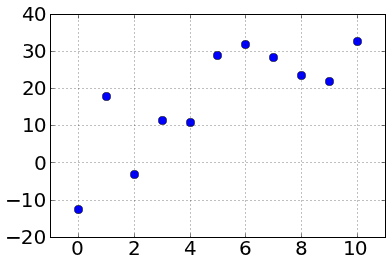
\includegraphics{img/fig1.png}

When we do a linear regression, we fit to a standard ``$y=mx+b$'' form.
For this data, the best fit is
\beqn
y=3.4 x + 0.27,
\eeqn
with a mean squared error of 77.9.  This difference from the line to the data is one measure of how well the line compares to the data - lower values means a better fit, a mean squared error of zero means a {\em perfect} fit.

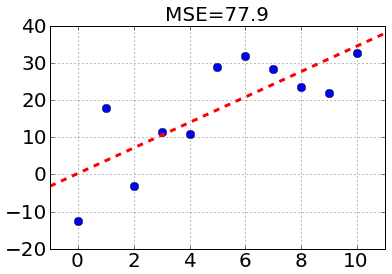
\includegraphics{img/fig2.png}

Overall, not a bad looking fit. However, if we fit to a more complex function, say a 10$^{\rm th}$ polynomial, we can get even better!

\beqn
y&=&-0.0007039 x^{10}  + 0.0363 x^9 - 0.8051 x^8 + 10.04 x^7 - 77.13 x^6 +\\
&& 376.5 x^5- 1159 x^4 + 2152 x^3 - 2163 x^2 + 891.8 x^1 - 12.54
\eeqn

with a Mean Squared Error of {\em zero}.

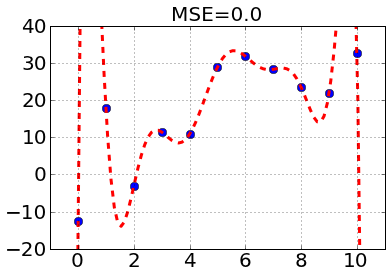
\includegraphics{img/fig4.png}

In the field of statistics, this is referred to as {\em over-fitting}, and is
the result of fitting the variation and not the overall pattern. In other words, it is fitting the
meaningless differences from one point to another by adding a tunable
parameter for each detail in the data. With each new parameter we get a
``better'' fit, by the criterion of mean squared error, but we lose
sight of the meaning. This is the mathematical equivalent of losing
sight of the forest for the trees.

\subsection{Parameters and Ockham's Razor}

When fitting a line, the result is choosing the values of the parameters that have the highest probability given the data.  However, when those parameters can take on any possible value, the overall probability of the model is reduced - this is the probabilistic equivalent of Ockham's Razor which we've seen before in Section~\ref{sec:ockham} on page~\pageref{sec:ockham}.  

We make the problem worse by adding more and more parameters, giving more possible explanatory freedom to our model.  The more freedom we have in choosing the parts of the model, the less explanatory power this model actually has.  One way that statisticians avoid this problem is to fit the model to half of the data, and see how it works on the other half - a process called cross-validation.  A simple model, like a straight line, will do about as well on both.  An overly complex one will do well on the data used to fit it, but will do poorly on new data.

\todo{do an example of this in this case}


\subsection{Back to the Resurrection}\label{back-to-the-resurrection}

If we look at Andy Bannister's very clever solution, we notice something
quite interesting: for every single difference between the Gospel
accounts, he adds a detail not found in the story to explain it. One can
pretty much do this for any two accounts that don't say logically
contradictory things, and can be seen as an example of over-fitting. 

Another way of looking at it is that, if Bannister had constructed his story from, say, two of the Gospel stories and then compared it to the other two he'd have a problem.  Even if he took details from all four accounts, but constructed a story from half of them and then used the other half to confirm it wouldn't work.

As a result, the Easter Challenge, as phrased, is probably not a very good one. One can Rube-Goldberg a story together to fit any amount of details.  Perhaps that is the point, to highlight to what lengths someone has to go to in order to reconcile the four accounts.  However, we think something motivated from cross-validation might be a bit more persuasive.
